\chapter{Structure of the code}
\label{appendix_structure}

The bulk of this manual is concerned with the available options to
build and run FHI-aims for a particular purpose. In our experience,
most users will probably remain at this level in their use of the
code, already due to the time constraints of a normal research
schedule. 

Nonetheless, we strongly believe that running a ``physics'' code as a
complete black-box package is not a good idea. Our branch of physics
is based on (mostly) well-understood differential equations, and the
solution technique applied, including its limitations, must be well
understood, or at least understandable, to gauge the outcome of a
particular calculation. In order to achieve this, the source code to
the method used must be available. While we do not expect most users
to go through the code in its entirety with a fine-tothed comb, we
\emph{do} encourage any user to look into the source code and try to
understand in which way FHI-aims produces its exact solution to a
problem. 

The purpose of this appendix is to facilitate this understanding, by
outlining the overall structure of the code, specifically, the
high-level subdivision of physical tasks.

\section{Flow of the program}

\begin{figure}
\begin{center}
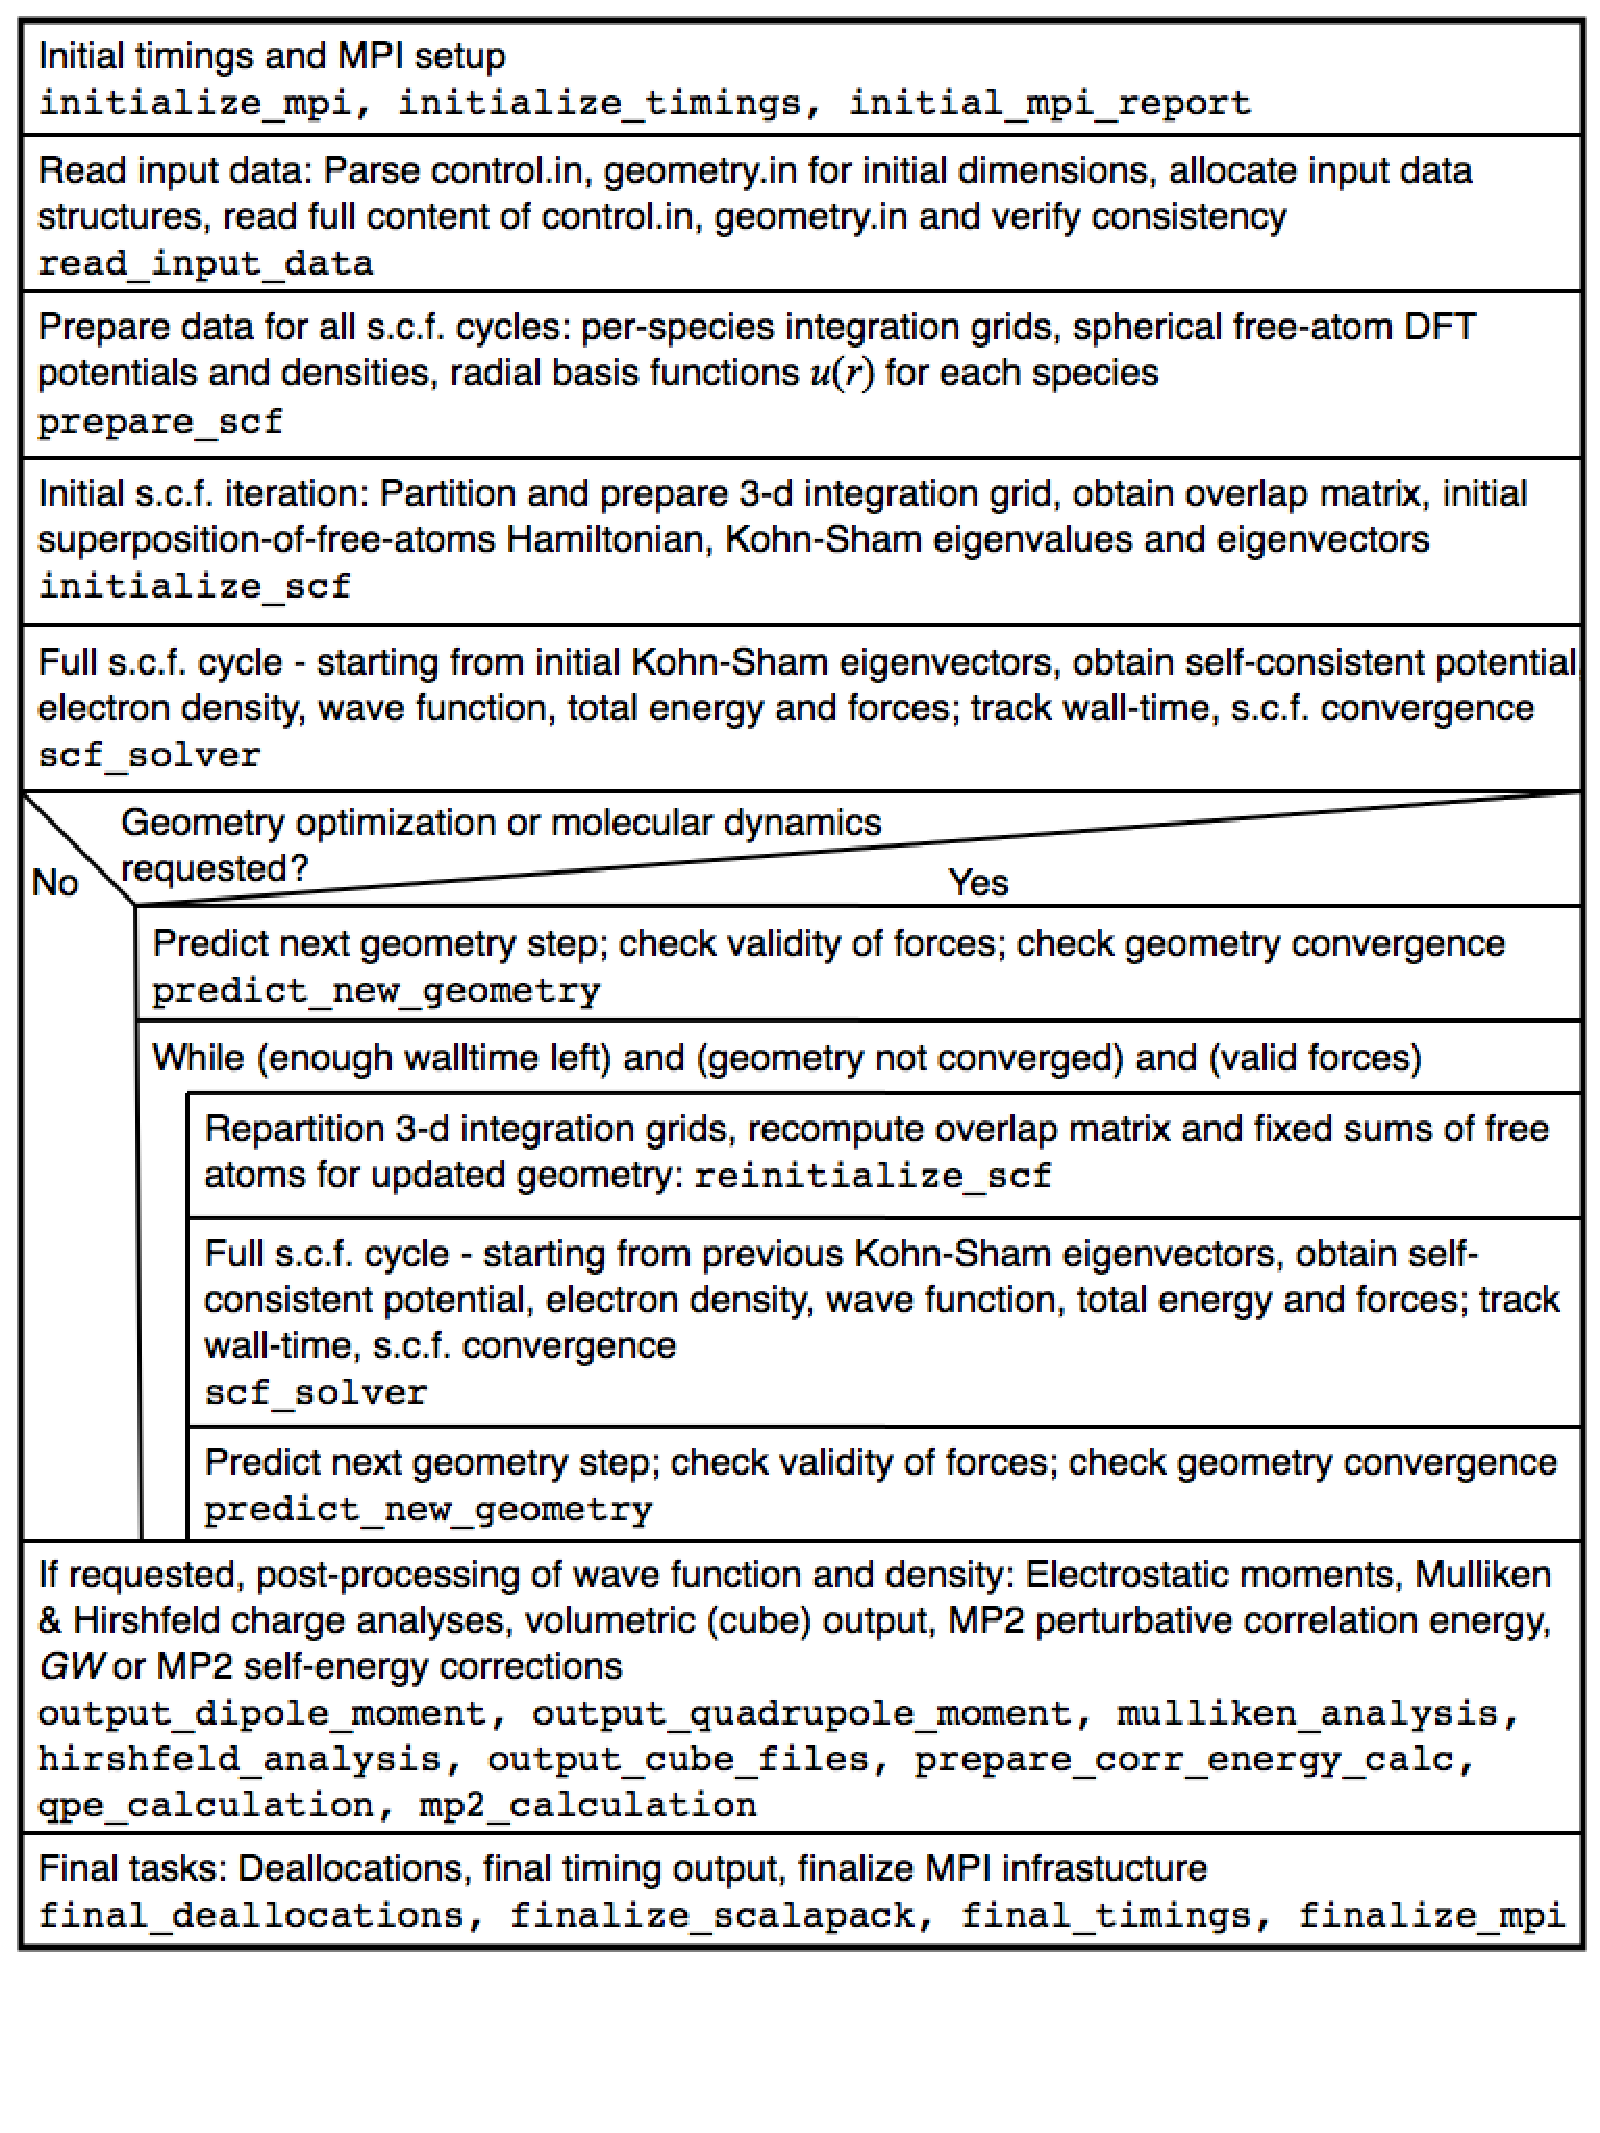
\includegraphics[height=0.9\textheight]{structogram_main}
\end{center}
\caption{High-level program flow of FHI-aims}
\label{Fig:main.f90}
\end{figure}

The uppermost level of FHI-aims is the subroutine \texttt{main.f90},
the structure of which is shown as a structogram in
Fig. \ref{Fig:main.f90}. As a subroutine, \texttt{main.f90} can also
be called by external code as a library subroutine, with the
restriction that, for parallel execution, this can happen only once
[by definition of the message passing interface (MPI) for parallel
communication, there can only be one call to \texttt{mpi\_init} per
program run]. 

The purpose of \texttt{main.f90} is to provide a logical separation of
groups of computational tasks by way of high-level wrapper subroutines
(listed in \texttt{typewriter} font in Fig. \ref{Fig:main.f90}). With
the exception of global convergence checks, no outright physical
quantities are directly manipulated in \texttt{main.f90}. All
physically relevant quantities are handled inside the lower-level
structure of the code and, if necessary, are passed between them by
way of specific modules. For example, the module \texttt{physics.f90}
handles all variables of tangible physical importance (Hamiltonian and
overlap matrices, Kohn-Sham wave function, electron densities,
potentials, ...). The geometry information for a given electronic
structure cycle (coordinates) are found in module
\texttt{geometry.f90}; etc. 

More details regarding these and other
modules are included with the code distribution as a separate
document. The point here is that \texttt{main.f90} should never need
to use any but the highest-level modules explicitly, i.e.:
\begin{itemize}
  \item \texttt{dimensions.f90} : Inclusion of array dimensions
    for consistent allocations across the code, and wrapper flags to
    prevent access to unallocated variables which are not needed for a
    given task.
  \item \texttt{localorb\_io.f90} : Wrapper module for consistent
    writing of output in parallel runs
  \item \texttt{mpi\_utilities.f90} : Wrapper module for MPI
    initialization, finalization (first and last tasks of a run,
    respectively), and task distribution
  \item \texttt{timing.f90} : Wrapper module including all timing and
    accounting information, including the count of s.c.f. iterations,
    relaxation or MD steps.
\end{itemize}

The first task of \texttt{main.f90} is to initialize any accounting
(timing etc.) information, the infrastructure required for MPI (or, to
silently switch off the use of MPI entirely in the case of
non-parallel runs), and to record all this information (initial time
stamps, code version, number of parallel tasks and computer system
layout) in the standard output.

The obvious next task is to read and process all input information
given in \texttt{control.in} and \texttt{geometry.in}. Internally,
this is handled in three steps (see the wrapper subroutine
\texttt{read\_input\_data.f90}): First, both input files are parsed once,
while extracting only the dimension information needed to set up any
necessary arrays / array dimensions needed to house the following
input data. Organizing this information is the task of module
\texttt{dimensions.f90}. Next, the information in \texttt{control.in}
is read and checked for consistency, using \texttt{read\_control.f90}
for all general information, and repeated calls to
\texttt{read\_species\_data.f90} for all \keyword{species}-related
information. Finally, subroutine \texttt{read\_geo.f90} reads the
input data of \texttt{geometry.in}, and verifies its consistency with
the data contained in \texttt{control.in}.

At the end of this step (subroutine \texttt{read\_input\_data.f90}),
\emph{all} input data from all input files should have been read and
processed. It is important that any known conflicts, or incomplete
settings, should have been verified at this stage, stopping the code
with an error message if outrightly conflicting input information is
detected. For completeness, we mention that any technical input
settings of global interest (e.g., the handling of spin, relativity,
or exchange-correlation) are collected and accessible through the
top-level module \texttt{runtime\_choices.f90}. 

The following steps are the ``household'' steps of electronic
structure theory. 

Wrapper subroutine \texttt{prepare\_scf.f90} sets up
all structure-independent, fixed pieces of the calculation, and stores
them for easy access in the actual self-consistency cycle. This
includes all free-atom quantities (densities and potentials for the
initialization), radial basis functions for all \keyword{species},
one-dimensional logarithmic and three-dimensional radial and angular
integration grids, and fixed coefficients for the analytic long-range
part of the Hartree potential.

Wrapper subroutine \texttt{initialize\_scf.f90} performs the initial
s.c.f. cycle of the electronic structure calculation. In this step,
the full three-dimensional integration grid is filled with fixed
initial quantities (superposition of free-atom densities, 
potentials, and partition functions), the overlap and Hamiltonian
matrix integrals are performed for the first time, and the initial
Hamiltonian and overlap matrices are used to determine the storage
requirements in the event of sparse matrix storage. If a two-electron
Coulomb operator is needed (hybrid functionals, Hartree-Fock, MP2,
$GW$ etc.), the three-center overlap matrix elements $(ij|\mu)$ of
Eq. (\ref{RI_V}) (see Sec. \ref{Sec:auxil} for details) and the
Coulomb matrix of the auxiliary ``resolution of the identity'' basis set
[denoted $V_{\mu\nu}$ in Eq. (\ref{RI_V})] are precomputed. 
The most important task in \texttt{initialize\_scf.f90} is the initial
solution of the Kohn-Sham equations Eq. (\ref{Eq:EVP}), providing a
first solution of the wave function coefficients $c_{jl}$. These are
the starting point of every iteration of the s.c.f. cycle in the
following step, subroutine \texttt{scf\_solver.f90}. 

With all preliminary information  available, the task of
\texttt{scf\_solver.f90} is to produce a self-consistent electron
density, wave function, and all associated observables for a given,
fixed nuclear geometry. The order of the cycle until convergence is
reached is: 
\begin{enumerate}
  \item Calculation of the Kohn-Sham electron density associated with the
    current wave function, $c_{jl}$ 
  \item electron density mixing and preconditioning, to produce the
    \emph{input} electron density for the next set of Kohn-Sham
    equations
  \item decomposition of the electron density into atom-centered
    multipole fragments $\delta\tilde{n}_{\text{at},lm}(r)$ [see
    Eq. (Eq;mp)], and construction of the multipole components of the
    Hartree potential, $\delta\tilde{v}_{\text{at},lm}(r)$
  \item construction of the full electrostatic potential
    $v_\text{es}(\boldr)$ on all points $\boldr$ of the
    three-dimension integration grid
  \item Integration of the updated Hamiltonian matrix elements,
    $h_{ij}$
  \item possible addition of two-electron exchange matrix elements to
    $h_{ij}$
  \item solution of the Kohn-Sham equations Eq. (\ref{Eq:EVP}), to
    produce an updated wave function $c_{jl}$
  \item computation of updated total energy components, and check of
    all convergence criteria.  
\end{enumerate}
After convergence is reached, \texttt{scf\_solver.f90} also performs
some inevitable post-processing steps, including ``scaled ZORA''
perturbative corrections for the appropriate relativistic treatment,
and band structure and density of states data output.

With a converged self-consistent solution at hand, the code can now
perform any number of similar calculations for updated geometries,
e.g., for a geometry optimization, molecular dynamics, etc. If so, an
updated geometry is first produced by subroutine
\texttt{predict\_new\_geometry.f90}. Note that this simple subroutine
should also serve as the starting point for any other calculations
involving multiple geometries, such as the calculation of ``serial''
geometries along a given set of coordinates, etc. For the updated
geometry, all geometry-related storage arrays in the calculation and
the overlap matrix must be recomputed in subroutine
\texttt{reinitialize\_scf.f90}. Following this, subroutine
\texttt{scf\_solver.f90} is invoked again, and a new self-consistent
solution is obtained. 

The final step of the code is to produce, by post-processing, any
information that can be obtained from the converged self-consistent
wave function or electron density, including electrostatic moments,
charge analyses, etc. Beyond this, only necessary cleanup tasks
follow, most notably the deallocation of all storage arrays and the
MPI infrastructure, and the final time accounting information. 

\section{Commenting and style requests}

Generally, no \emph{strong} style conventions are enforced within
FHI-aims, recognizing the fact that most programmers follow their own
style conventions and preferences when it comes to details. There are,
however, some conventions that should be followed in order to keep the
code as a whole legible, and maintainable. When writing additional
code, please adhere to these, using existing modules or subroutines as
models where appropriate.

\textbf{A current set of ``code conventions'' is maintained at the Wiki
  at aimsclub.} A subset of these recommendations includes:
\begin{enumerate}
  \item Please comment your work. Any necessary functionality should
    be accompanied with comments, enough so that \emph{at least}
    someone familiar with the underlying mathematics can follow your
    code. 
  \item Please provide regular comment headers for your work. Every
    module and subroutine comes with comment headers in the style used
    by the \emph{Robodoc} code management system (see, e.g.,
    \url{http://www.xs4all.nl/~rfsber/Robo} for details and a
    manual). Beyond the possible use of Robodoc, we follow this
    convention because it provides a clear and unambiguous laundry
    list of items that are needed in any subroutine header: a
    description of the subroutine \emph{purpose}, possibly its
    \emph{input} and \emph{output} data, and most importantly a
    \emph{copyright} statement that is needed for every file in the
    code distribution. 
  \item Please keep your usage of Fortran conservative. Some ambitious
    constructs, while desirable when following formal techniques such
    as fully object-oriented programming, can still expose
    compiler bugs when too ``un-Fortran-like'' syntax is used. 
  \item In particular, compiler-dependent bugs are the reason why the
    use of pointers is strongly discouraged in FHI-aims. Even when
    following the textbook, allocating and deallocating pointers works
    differently with different compilers, opening the possibility of
    unexpected memory leaks outside our control. Please don't do it ---
    this problem \emph{has} bitten us before.
\end{enumerate}
Again, please consult the ``aimsclub'' wiki for the full and current
recommended code conventions.
